\section{Stream Processing Languages}\label{sec:languages}

\begin{alltt}TODO\scriptsize ~6 pages total
- this section discusses 7 styles of streaming languages
  - ~0.75 pages and ~8 citations for each language style
  - each of these snippets structured around questions:
    why-who-when-what-where-whence
- before the snippets on each of the languages/styles, we will
  briefly introduce and explain these questions, as follows:
  - why: objective, audience, domain
  - who: inventors, supporters
  - when: first release / first paper
  - what: key idea, data model, type system, code example
  - where: being developed or offered today, license
  - whence: influenced-by and influences
- descriptions of individual language styles
\end{alltt}

\begin{figure}[!h]
\begin{lstlisting}
SELECT IStream(Max(len) AS mxl,
                 MaxCount(len) AS num,
                 ArgMax(len, caller) as who)
FROM Calls[Range 24 Hours Slide 1 Minute]
\end{lstlisting}
\vspace*{-4mm}
\caption{\label{fig:cql}CQL code example.}
\end{figure}

\begin{figure}
\centerline{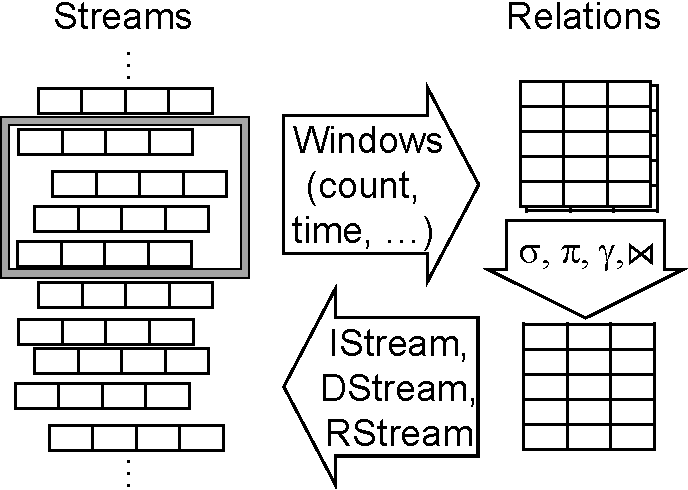
\includegraphics[scale=0.5]{cqlops.pdf}}
\vspace*{-4mm}
\caption{\label{fig:cqlops}CQL algebra operators.}
\end{figure}

\textbf{Relational Streaming.}
In 2004, Arasu et al.\ at Stanford introduced CQL (for Continuous
Query Language)~\cite{arasu_widom_2004}. CQL has been designed as an
SQL-based declarative language for implementing continuous queries
against streams of data, such as the LinearRoad
benchmark~\cite{arasu_et_al_2004}. The design was influenced by the language of
the TelegraphCQ system that proposed a declarative language with a
particular focus on expressive windowing
constructs~\cite{chandrasekaran_et_al_2003}. The semantics of CQL are
based on two data types: \emph{streams} and \emph{relations}. It
supports three classes of operators over these types. First,
\emph{stream-to-relation} operators, which produce a relation from a
stream.  The design of these operators is based on the concept of a
\emph{window} over a stream, which, at any point of time, contains a
historical snapshot of a recent portion of the stream. CQL includes
time-based and tuple-based windows, both with optional
partitioning. Second, \emph{relation-to-relation} operators, which
produce a relation from other relations. These operators are derived
from traditional relational algebra and are expressed using standard
SQL. Third, \emph{relation-to-stream} operators, which produce a
stream from a relation. CQL supports three operators of this class:
IStream, DStream, and RStream (to capture inserts, deletes, or the
relation).  Figure~\ref{fig:cql} illustrates a CQL code example that
uses a time-sliding window (per minute within the last 24 hours) over
phone calls to return the maximum phone call length along with its
count and caller information. CQL has influenced the design of many
systems such as Microsoft StreamInsight~\cite{ali_et_al_2009}.

GSQL~\cite{cranor_et_al_2003} is another streaming  language with SQL-like syntax.
It has been designed in the context of the Gigascope system~\cite{cranor2003gigascope}, a stream database for network applications
including traffic analysis, intrusion detection, router configuration analysis and network monitoring.
In GSQL, all queries operate over streams, as inputs and outputs. 
In addition to the standard SQL operator (e.g., selection, projection, join, aggregation), GSQL supports  the \emph{merge} operator that combines streams from multiple sources into a single stream. It acts as a union operator that preserves the \emph{ordering} properties of an attribute.
GSQL supports the join of two streams as long as it can determine
a join window from the join predicates. However, GSQL does
not support the join of a stream to a non-stream relation.


\begin{figure}[!h]
\begin{lstlisting}
node tracker (speed, limit: int) returns (t: int);
var x: bool; cpt: int when x;
let
  x = (speed > limit);
  cpt = counter((0, 1) when x);
  t = current(cpt);
tel
\end{lstlisting}
\vspace*{-4mm}
\caption{\label{fig:lustre} Lustre code example.}
\end{figure}

\textbf{Synchronous Dataflow.}
Dataflow synchronous languages were introduced to ease the design of
real-time embedded systems. They allow to write a well-defined
deterministic specification of the system. It is then possible to
test, verify, and generate embedded code.
The first dataflow synchronous languages Lustre~\cite{lustre_1987}
(Caspi and Halbwachs) and Signal~\cite{signal_1991} (Le Guernic,
Benveniste, and Gautier) were proposed in France in the late 80s.
A dataflow synchronous program is a set of equations defining streams
of values. Time proceeds by discrete logical steps, and at each step,
the program computes the value of each stream depending on its inputs
and possibly previously computed values.
This approach is reminiscent of block diagrams, a popular notation to
describe control systems.
Figure~\ref{fig:lustre} presents a Lustre code example that tracks the
number of times the speed of a vehicle exceeds the speed limit. The
counter \lstinline{cpt} starts with~$0$ and is incremented by~$1$ each
time the current speed exceed the current limit (\lstinline{when x}).
The return value \lstinline{t} maintain the last computed value
of \lstinline{cpt} between two occurrences of~\lstinline{x}
(\lstinline{current(cpt)}).
The dataflow synchronous approach has inspired
multiple languages: Lucid Synchrone~\cite{lucid_2006} combines the
dataflow synchronous approach with functional features \`a la ML,
StreamIt~\cite{streamit_2002} focuses on efficient processing of large
streaming applications, Z\'elus~\cite{zelus_2013} is a Lustre-like
language extended with ordinary differential equations to define
continuous-time dynamics. Lustre is also the backbone of the
industrial language and compiler Scade~\cite{scade_2017} routinely
used to program embedded controllers in many critical applications.

\begin{figure}[!h]
\begin{lstlisting}
stream<float64 len, rstring caller> Calls = CallsSrc() {}
type StatsT = tuple<float64 len, int32 num, rstring who>;
stream<StatsT> StatsS = Aggregate(Calls) {
   window Calls: sliding, time(24.0*60.0*60.0), time(60.0);
   output StatsS: len = Max(Calls.len),
                  num = MaxCount(Calls.len),
                  who = ArgMax(Calls.len, Calls.caller);
}
\end{lstlisting}
\vspace*{-4mm}
\caption{\label{fig:spl}SPL code example.}
\end{figure}

\textbf{Big-Data Streaming.}
%
The need to handle diverse data and processing needs at scale
motivated several recent big-data streaming languages and
systems~\cite{carbone_et_al_2015,hirzel_schneider_gedik_2017,toshniwal_et_al_2014,zaharia_et_al_2013}.
Each of them makes it easy to integrate operators written in
general-purpose languages and to parallelize them on clusters of
multicore computers. Hirzel et al.\ introduced the SPL
language~\cite{hirzel_schneider_gedik_2017} as part of the IBM~Streams
product in~2010. Figure~\ref{fig:spl} shows an example for a similar
use-case as Figure~\ref{fig:cql}. Line~1 defines a stream
\lstinline{Calls} by invoking an operator \lstinline{CallsSrc}, and
\mbox{Lines 3-8} define a stream \lstinline{StatsS} by invoking an
operator \lstinline{Aggregate}. An SPL program explicitly specifies a
directed graph of stream edges and operator nodes. Streams carry
tuples; in the examples, tuple attributes contain primitive values,
but in general, they can also contain compound values such as other
tuples or lists.  Operators create and transform streams; operators
are defined by users or libraries, not built into the
language. Operators can be further configured upon invocation, for
example, with windows or output assignments. To facilitate
distribution, SPL's semantics are defined to require minimal
synchronization between operators~\cite{soule_et_al_2016}. One can
view Borealis as the evolutionary link between relational streaming
and big-data streaming languages~\cite{abadi_et_al_2005}. In the
big-data domain, SPL has been followed by
Storm~\cite{toshniwal_et_al_2014}, Spark
Streaming~\cite{zaharia_et_al_2013}, Flink~\cite{carbone_et_al_2015},
and others.

\begin{alltt}TODO\scriptsize Martin
- more extensively describe Storm, Spark, and Flink
\end{alltt}

\begin{figure}[!h]
\begin{lstlisting}
/* Either from similar domain as CQL example:
  alert when calls from locations over
  10 miles apart within 60 seconds. */
stream<Alert> Alerts = MatchRegex(Calls) {
  param
    partitionBy: caller;
    pattern    : ".+ tooFarTooFast";
    predicates : {
      tooFarTooFast =
            geoDist(First(loc), Last(loc)) >= 10.0
        && timeDist(First(ts), Last(ts)) <= 60.0; };
  output
    Alerts: who=caller, where=Last(loc), when=Last(ts);
}
/* Or from similar domain as Lustre example:
   simple edge detector, each time a car's speed
   increases over the speed limit, emit a tuple
   with a count of 1. */
stream<Edge> Edges = MatchRegex(CarUpdates) {
  param  pattern    : "below above";
         partitionBy: car;
         predicates : { below = speed <= limit;
                        above = speed > limit; };
  output Edge: car=car, speed=Max(speed), count=1;
}
\end{lstlisting}
\vspace*{-4mm}
\caption{\label{fig:cep}CEP example.}
\end{figure}

\textbf{Complex Event Processing.}
%
Complex Event Processing (CEP) is another technology with respect to stream processing, which is oftentimes
considered as an alternative or as a special case of stream processing. The latter thesis has led to define CEP
operators in classical streams processing languages. A prominent example on top of SPL~\cite{hirzel_schneider_gedik_2017} described above is the
MatchRegex~\cite{hirzel_2012} operator, whose implementation is available in the System S distributed streaming platform. This operator has been introduced by Hirzel in 2012 and influenced by the MATCH-RECOGNIZE~\cite{zemke_et_al_2007} version, which is part of the SQL ANSI
standard. With respect to its SQL counterpart,  MatchRegex is much more simplified and concise in terms of syntax as well as easy to deploy as a library operator.
Figure~\label{fig:cep} shows an example of SPL source code with MatchRegex operator.
It permits to capture a composite event in which the speed of a vehicle already overcoming the limit rises beyond the maximum value of the speed
observed so far (corresponding to the first predicate rise). This event can be repeated several times due to the presence of the Kleene-plus in the regular expression of the pattern. Similarly,
the minimum speed registered within the speed bound is captured in the second predicate and its value is provided as output, along with the number of times when these rises and drops occurs and the first
foreseen event of either kind. The MatchRegex~\cite{hirzel_2012} operator is implemented via code generation and translates to an automaton, which permits space and time-efficient incremental computation of aggregates. Other functionalities beyond pattern matching are not supported, such as join operations and reporting tasks.

%\begin{alltt}TODO\scriptsize, ~0.75 pages, ~8 citations, \textcolor{red}{Angela}
%- e.g. MATCH-RECOGNIZE \cite{zemke_et_al_2007}, MatchRegex \cite{hirzel_2012}
%\end{alltt}

\begin{figure}[!h]
\begin{lstlisting}
CREATE ~\textit{cq\_name}~
         ~\textit{xml\_ql\_query}~
     DO ~\textit{action}~
  {START ~\textit{start\_time}~}
  {EVERY ~\textit{time\_interval}~}
  {EXPIRE ~\textit{expiration\_time}~}
\end{lstlisting}
\vspace*{-4mm}
\caption{\label{fig:Niagra}NiagaraCQ code example.}
\end{figure}

\textbf{XML Streaming.}
Chen et al.\ introduced NiagaraCQ~\cite{chen_et_al_2000} in 2000 as a
continuous query sub-system of the Niagara internet query engine, a
data\-base for querying distributed XML data sets developed at
University of Wisconsin and Oregon Graduate
Institute~\cite{naughton2001niagara}. NiagaraCQ implements continuous
query processing over XML files by supporting incremental evaluation
and considering only the changed portion of each updated XML file. It
supports two types of continuous queries that differ in the criteria
triggering their execution: \emph{change-based} queries, which trigger
as soon as new relevant data becomes available, and \emph{timer-based}
queries, which trigger only at specified time intervals.  NiagaraCQ is
based on XML-QL~\cite{deutsch1999query}.  It provides a command
language for creating continuous queries that follows the form
illustrated in Figure~\ref{fig:Niagra}. Using this command language,
users can implement continuous queries that combines an ordinary
XML-QL query with additional time information.  The
\textsf{\small\textit{xml\_ql\_query}} becomes effective at the
defined \textsf{\small\textit{start\_time}}.  The
\textsf{\small\textit{time\_interval}} indicates how often the query
will be executed. A query is timer-based if its
\textsf{\small\textit{time\_interval}} is non-zero; otherwise, it is
change-based.  The continuous query will be deactivated after its
\textsf{\small\textit{expiration\_time}}. The
\textsf{\small\textit{action}} triggers once the results of the XML-QL
query expression is returned.  A key optimization mechanism used in
the NiagaraCQ system is grouping the execution of similar queries to
minimize redundant work.  YFilter~\cite{diao_et_al_2002,diao2003high} implements
continuous queries based on XPath~\cite{clark_derose_1999}, also with
multi-query optimization. The main idea of YFilter is to use a single
finite state machine to represent and evaluate several XPath
expressions. In particular, YFilter exploits the commonality among path queries by merging the common prefixes
of the paths so that they are processed at most once. This  shared processing mechanism provides significant performance
improvement by avoiding redundant processing for duplicate path expressions. In order to handle value-based predicates that address contents of elements, YFilter applies two alternative approaches. The first approach approach evaluates the  predicates once the addressed elements are read from a document, while the other approach postpones predicate evaluation until the corresponding path expression has been entirely matched.


\begin{figure}[!h]
\begin{lstlisting}
TODO: RDF streaming example
\end{lstlisting}
\vspace*{-4mm}
\caption{\label{fig:rdf}RDF streaming example.}
\end{figure}

\textbf{RDF Streaming.}
\begin{alltt}TODO\scriptsize, ~0.75 pages, ~8 citations, \textcolor{red}{Emanuele, Akrivi}
- e.g., C-SPARQL \cite{barbieri_et_al_2009}
- stream reasoning (either separate snippet, or included here)
\end{alltt}

\begin{figure}[!h]
\centerline{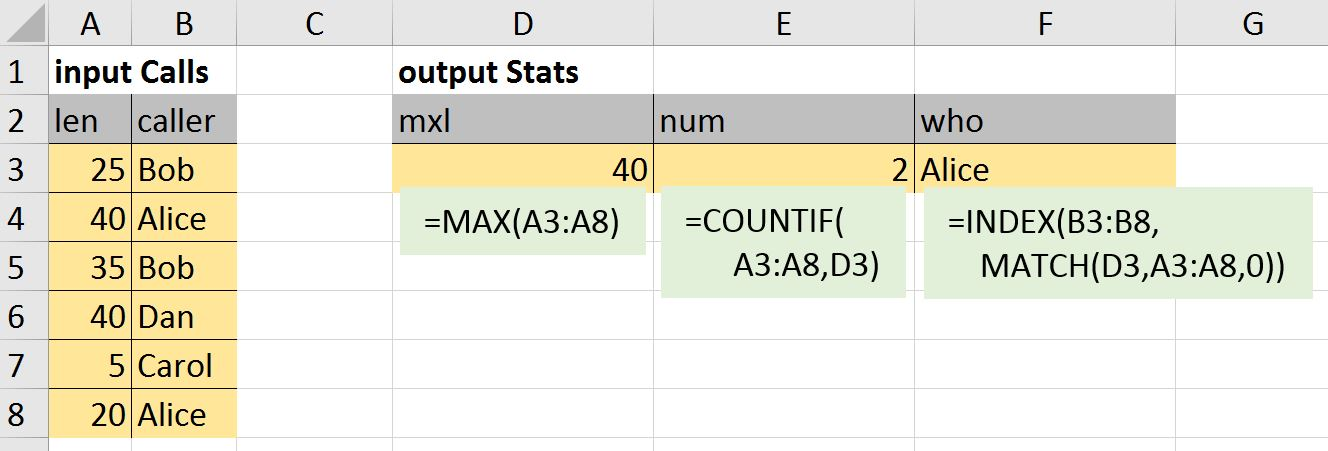
\includegraphics[width=\columnwidth]{CallStats.jpg}}
\vspace*{-4mm}
\caption{\label{fig:activesheets}ActiveSheets example.}
\end{figure}

\textbf{Streaming for End-Users.}
%
We use the term \emph{end-users} to refer to users without particular
software development training. Probably the most successful
programming tool for end-users is spreadsheet formulas. And from the
early days of VisiCalc in 1979~\cite{bricklin_frankston_1979},
spreadsheet formulas have been \emph{reactive} in the sense that any
changes in their inputs trigger an automatic recomputation of their
outputs. Therefore, in 2014, Vaziri et al.\ designed ActiveSheets, a
spreadsheet-based stream programming model~\cite{vaziri_et_al_2014}.
Figure~\ref{fig:activesheets} gives an example that implements a
similar computation as Figures \mbox{\ref{fig:cql} and \ref{fig:spl}}.
Cells \lstinline{A3:B8} contain a sliding window of recent call
records, which ActiveSheets updates from live input data. Cells
\lstinline{D6:F6} contain the output data, \mbox{(re-)}com\-pu\-ted
using reactive spreadsheet formulas. The formula
\mbox{\lstinline{E6=COUNTIF(A3:A8,D6)}} counts how many calls in the
window are as long as a longest call. The formula
\mbox{\lstinline{F6=INDEX(B3:B8,F2)}} uses the relative index \lstinline{F2}
of the longest \lstinline{len} to retrieve the corresponding
caller.  ActiveSheets was influenced by
synchronous data\-flow~\cite{lustre_1987} and has been extended with
time-based windows, key-based partitions, and performance
optimizations~\cite{hirzel_et_al_2016}. Other ideas besides
spreadsheets that have been used to let end-users build streaming
applications include trigger-action programming~\cite{ifttt} and
controlled natural language~\cite{arnold_et_al_2016}.

\textbf{Summary.}
\begin{alltt}TODO\scriptsize
- close with comparison table?
- perhaps according to performance/generality/productivity
\end{alltt}
